
\usetikzlibrary{calc,decorations.pathmorphing,shapes,positioning}
\newcounter{sarrow}
\newcommand\xrsquigarrow[1]{%
\stepcounter{sarrow}%
\mathrel{\begin{tikzpicture}[baseline= {( $ (current bounding box.south) + (0,-0.5ex) $ )}]
\node[inner sep=.5ex] (\thesarrow) {$\scriptstyle #1$};
\path[draw,<-,decorate,
  decoration={zigzag,amplitude=0.7pt,segment length=1.2mm,pre=lineto,pre length=4pt}]
    (\thesarrow.south east) -- (\thesarrow.south west);
\end{tikzpicture}}%
}
\makeatletter
\newcommand{\xRightarrow}[2][]{\ext@arrow 0359\Rightarrowfill@{#1}{#2}}
\makeatother

\newcommand{\thmref}[1]{\cref{#1}~(\nameref{#1})}
\newcommand{\Thmref}[1]{\Cref{#1}~(\nameref{#1})}

\newcommand*{\incompleteproofname}{Proof}
\newenvironment{incompleteproof}[1][\incompleteproofname]{\begin{proof}[#1]\renewcommand*{\qedsymbol}{{\faIcon{hat-wizard}}}}{\end{proof}}

%%%%
% TODO macros
\newcommand{\MK}[1]{\todo[color=orange!30]{TODO: #1}}
\newcommand{\MKin}[1]{\todo[color=orange!30,inline]{TODO: #1}}
\newcommand{\MP}[1]{\todo[color=blue!30]{TODO: #1}}
\newcommand{\MPin}[1]{\todo[color=blue!30,inline]{TODO: #1}}
\newcommand{\MPpost}[1]{\todo[color=yellow!30,inline]{TODO: #1}}
\newcommand{\hltt}[1]{\begin{center}\fbox{\color{green}\large{#1}}\end{center}}

% Approx
\newcommand{\pages}[1]{}%\xspace\todo{\textbf{($\sim$#1 pages)}\xspace}}

%%%%
% Colors
\newcommand{\neutcol}[0]{black}
\newcommand{\stlccol}[0]{RoyalBlue}
\newcommand{\irccol}[0]{Apricot}
\newcommand{\ulccol}[0]{RedOrange}
\newcommand{\objcol}[0]{Emerald} %CarnationPink}
\newcommand{\commoncol}[0]{black}

\newcommand{\col}[2]{\ensuremath{{\color{#1}{#2}}}}

\newcommand{\com}[1]{\ensuremath\mathit{\col{\neutcol}{#1}}}
\newcommand{\src}[1]{\ensuremath\mathsf{\col{\stlccol}{#1}}}
\newcommand{\irl}[1]{\ensuremath\mathit{\col{\irccol}{#1}}}
\newcommand{\trg}[1]{\ensuremath\mathbf{\col{\ulccol}{#1}}}
\newcommand{\obj}[1]{\ensuremath\mathtt{\col{\objcol}{#1}}}

%%%%
% Text Decorations
\newcommand\BrText[2]{%
  \par\smallskip
   \noindent\makebox[\textwidth][r]{$\text{\scriptsize #1}\left\{
    \begin{minipage}{\textwidth}
    #2
    \end{minipage}
  \right.\nulldelimiterspace=0pt$}\par\smallskip
}
\newcommand{\mi}[1]{\ensuremath{\mathit{#1}}}
\newcommand{\mr}[1]{\ensuremath{\mathrm{#1}}}
\newcommand{\mt}[1]{\ensuremath{\texttt{#1}}}
\newcommand{\mtt}[1]{\ensuremath{\mathtt{#1}}}
\newcommand{\mf}[1]{\ensuremath{\mathbf{#1}}}
\newcommand{\mk}[1]{\ensuremath{\mathfrak{#1}}}
\newcommand{\mc}[1]{\ensuremath{\mathcal{#1}}}
\newcommand{\ms}[1]{\ensuremath{\mathsf{#1}}}
\newcommand{\mb}[1]{\ensuremath{\mathbb{#1}}}
\newcommand{\msc}[1]{\ensuremath{\mathscr{#1}}}

\newcommand{\bul}[1]{{\setulcolor{RoyalBlue}\ul{#1}}}
\newcommand{\rul}[1]{{\setulcolor{RedOrange}\ul{#1}}}
\newcommand{\iul}[1]{{\setulcolor{Apricot}\ul{#1}}}
\newcommand{\oul}[1]{{\setulcolor{Emerald}\ul{#1}}}
\newcommand{\pul}[1]{{\setulcolor{CarnationPink}\ul{#1}}}

\newcommand{\lock}{\ensuremath\text{\scriptsize\faIcon{lock}}}
\newcommand{\unlock}{\ensuremath\text{\scriptsize\faIcon{lock-open}}}

\newcommand{\tup}[2]{\ensuremath (#1 %
  \readlist\myterms{#2}%
  \foreachitem\x\in\myterms{;\x}%
  )%
}

\newcommand{\isdef}[0]{\ensuremath{\mathrel{\overset{\makebox[0pt]{\mbox{\normalfont\tiny\sffamily def}}}{=}}}}

%%%%
% List of contributions
\newcounter{contrib}
\newcommand{\contribnum}[0]{\stepcounter{contrib}{\arabic{contrib}}.~}
\newcommand{\contribution}[1]{\smallskip\noindent\textbf{{#1.}\xspace}}

%%%%
% A symbol for Coq-verified theorems.
\newcommand{\BareCoqSymbol}{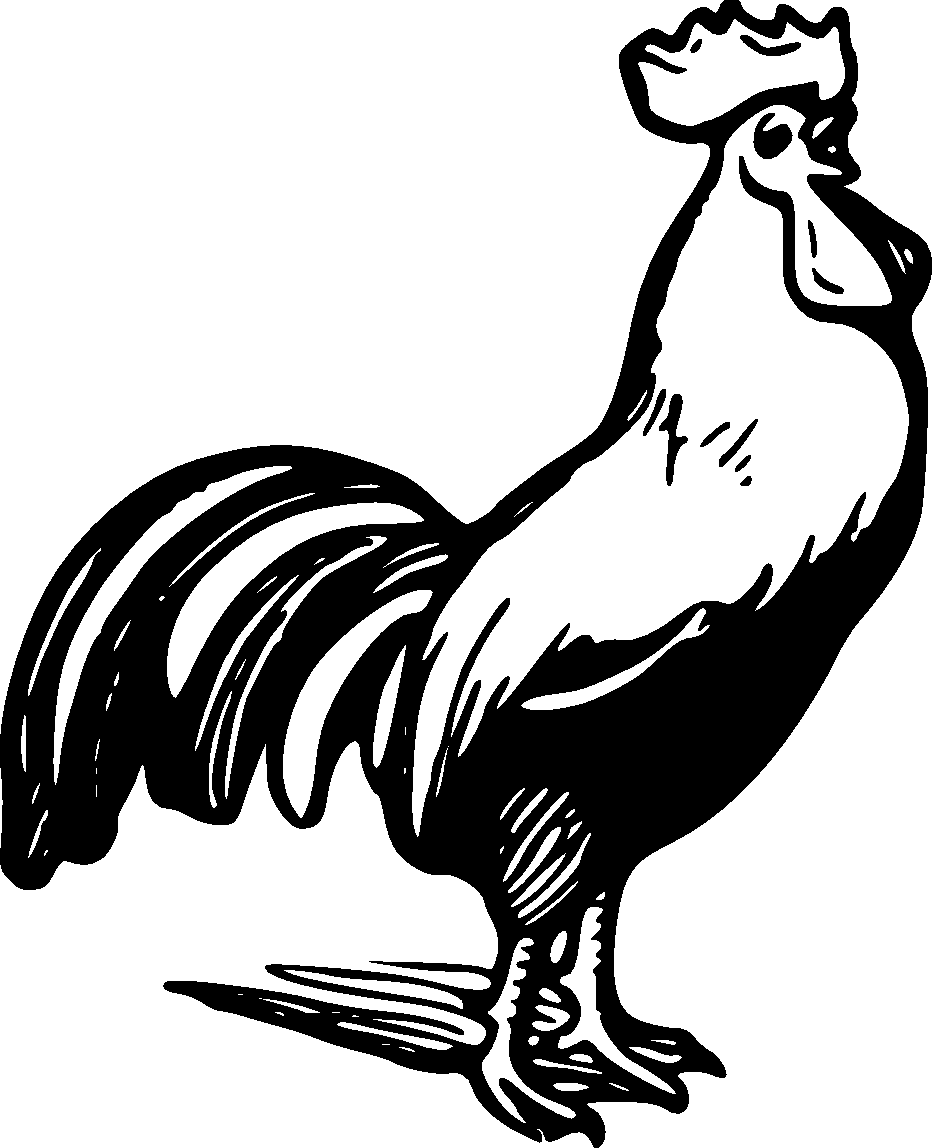
\includegraphics[height=0.9em]{coq.pdf}}
\newcommand{\CoqSymbol}{\raisebox{-.2ex}{\BareCoqSymbol\,}}
\newcommand{\Coqed}{\hfill\CoqSymbol}

\newcommand{\BareInvCoqSymbol}{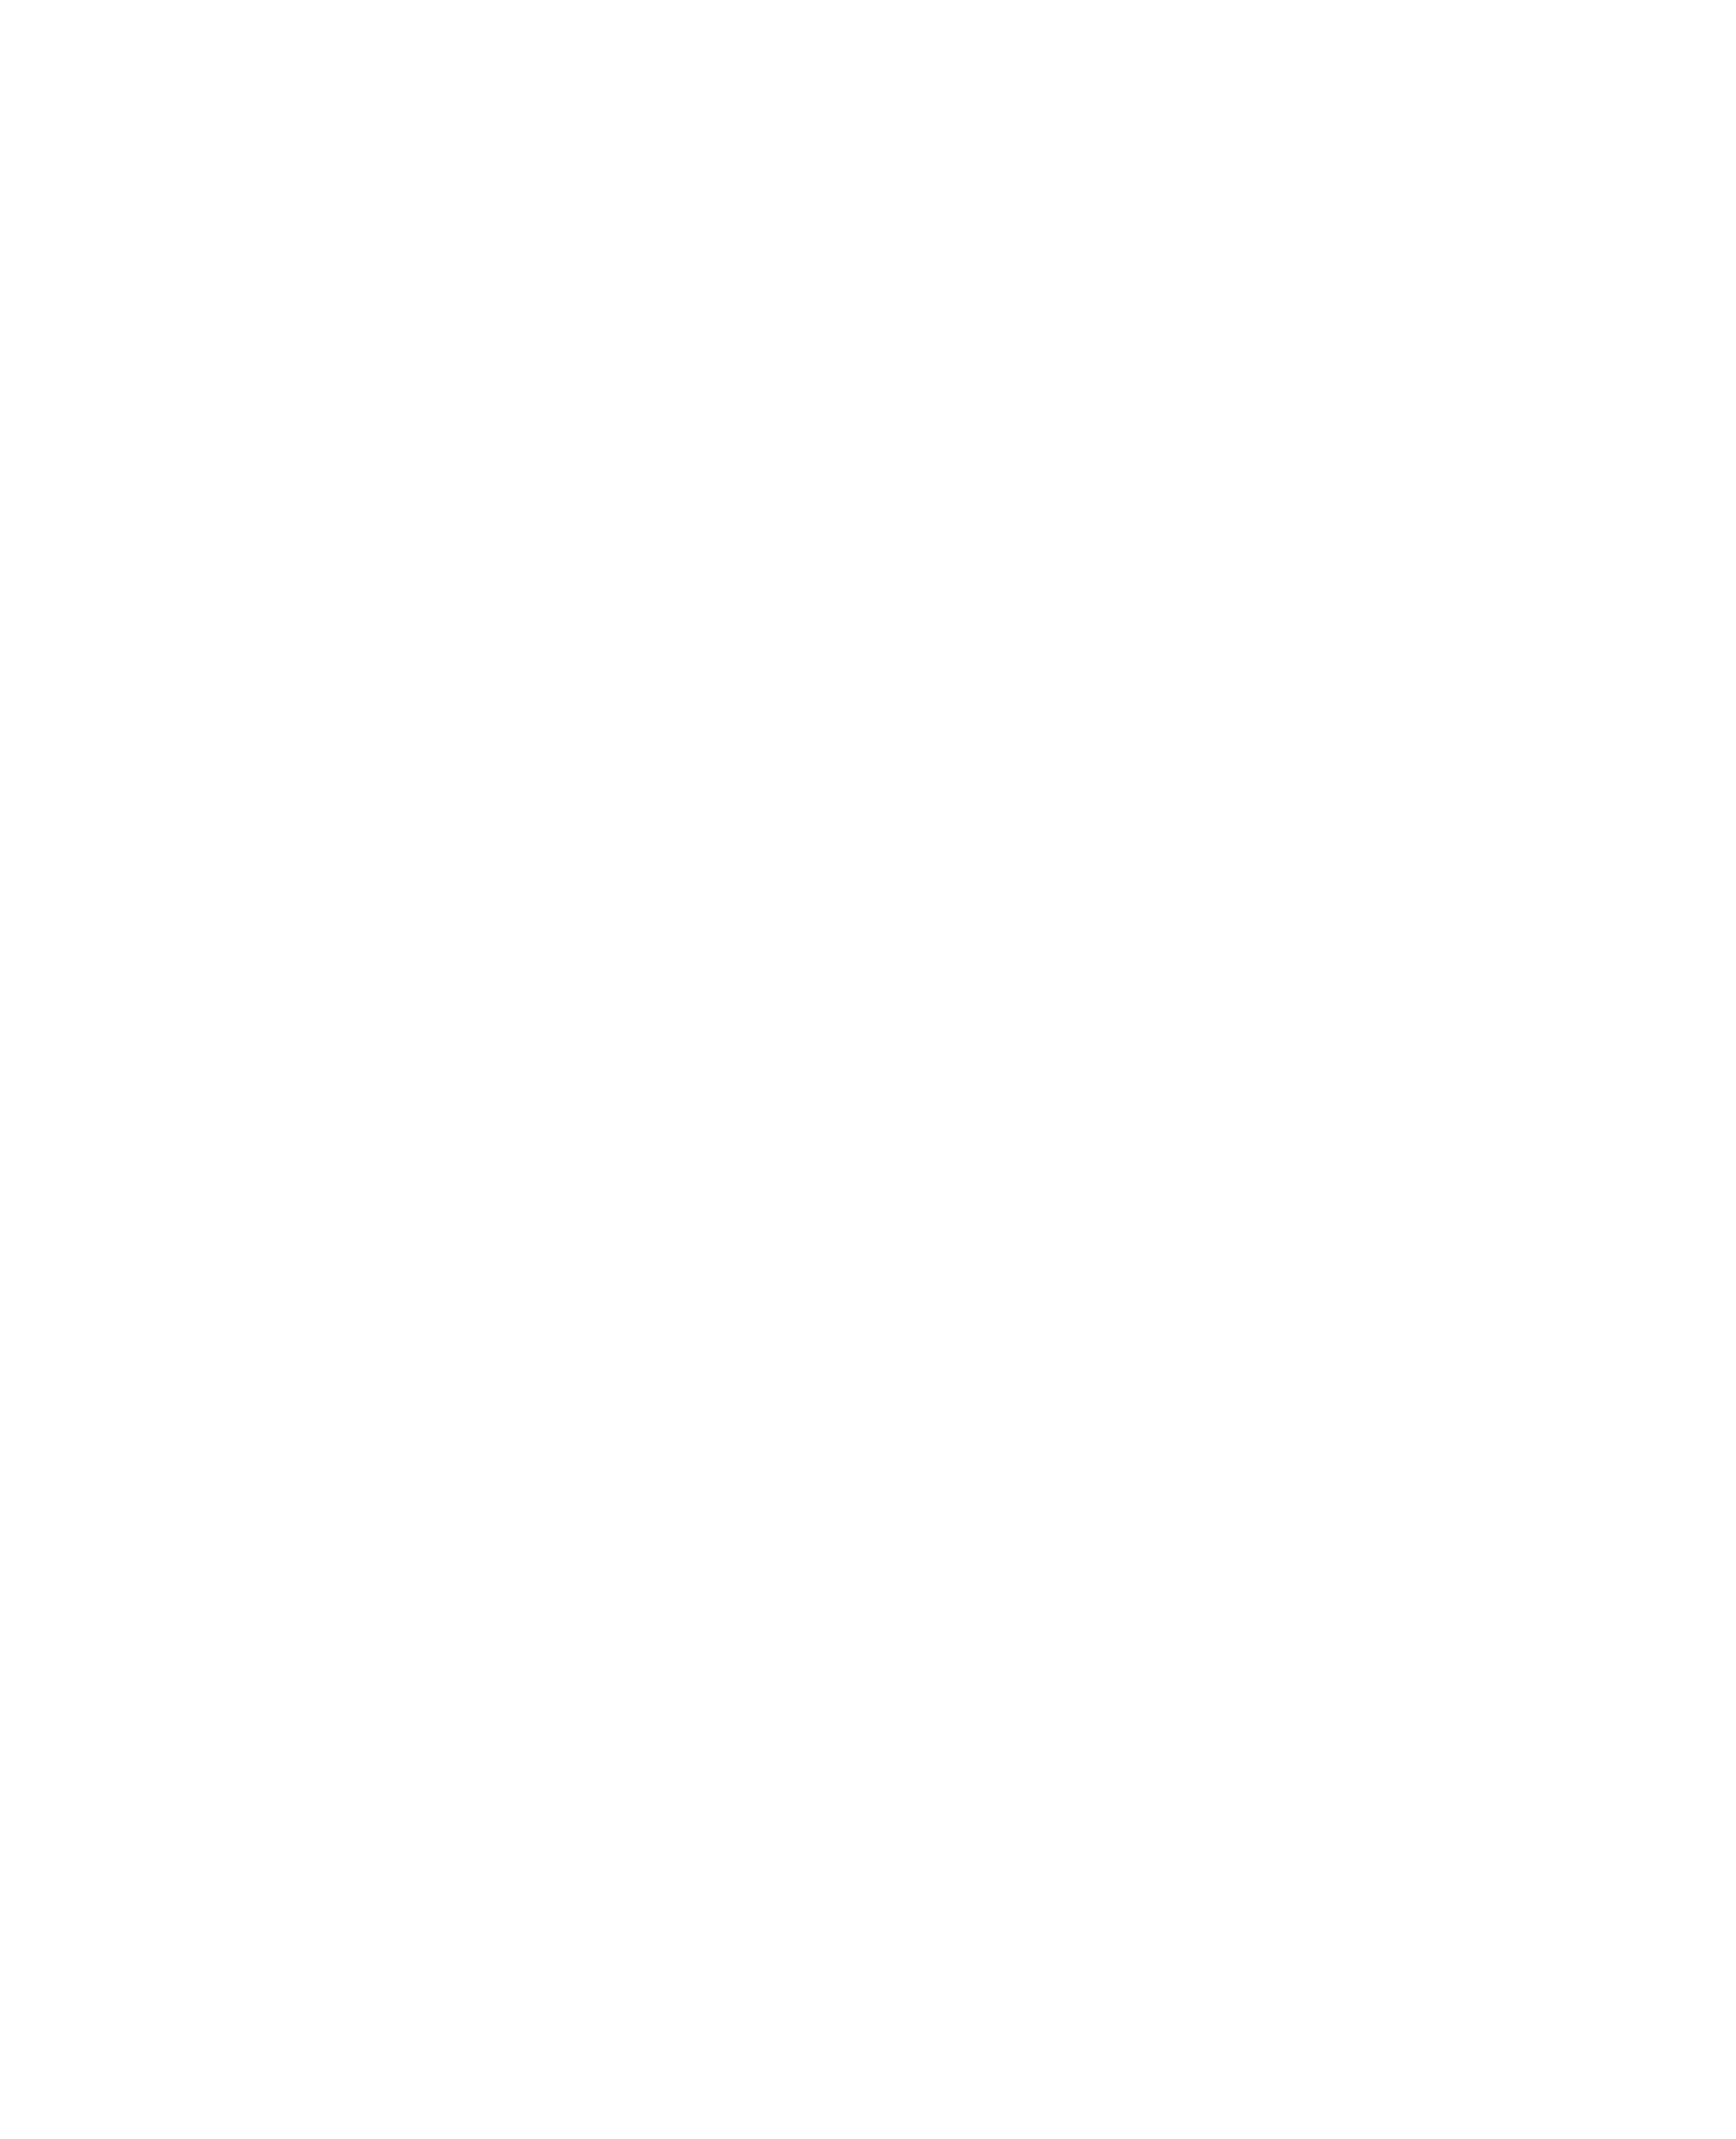
\includegraphics[height=0.9em]{inv_coq.png}}
\newcommand{\InvCoqSymbol}{\raisebox{-.2ex}{\BareInvCoqSymbol\,}}

%%%%
% Typerules
\newcommand{\textgraybox}[1]{\boxed{#1}}
\newdimen\zzfontsz
\newcommand{\fontsz}[2]{\zzfontsz=#1%
{\fontsize{\zzfontsz}{1.2\zzfontsz}\selectfont{#2}}}
\newcommand{\mathsz}[2]{\text{\fontsz{#1}{$#2$}}}
\newcommand{\instsymColon}{%
     \raisebox{-0.09ex}{\text{\normalfont{:}}}}
\newcommand{\judgboxfontsize}[1]{%
        \mathsz{11pt}{#1}%
}
\newcommand{\judgbox}[2]{%
      {\raggedright \textgraybox{\ensuremath{\judgboxfontsize{#1}}}\!%
        \fontsz{9pt}{\begin{tabular}[c]{l} #2 \end{tabular}} %
}}
\newcounter{typerule}
\crefname{typerule}{rule}{rules}

\newcommand{\typeruleInt}[5]{%
	\def\thetyperule{#1}%
	\refstepcounter{typerule}%
	\label{tr:#4}%
	%
  \ensuremath{\begin{array}{c}#5 \inference{#2}{#3}\end{array}}
}
\newcommand{\typerule}[4]{%
  \typeruleInt{#1}{#2}{#3}{#4}{\textsf{\scriptsize ({#1})} \\      }
}
\newcommand{\typerulenolabel}[3]{%
	\def\thetyperule{#1}%
	\refstepcounter{typerule}%
  \ensuremath{\begin{array}{c} \inference{#2}{#3}\end{array}}
}
\newcommand{\typerulederiv}[3]{%
  \ensuremath{\begin{array}{c} \inference{#2}{#3} #1\end{array}}
}

%%%%
% Language-specific definitions
% names of properties
\newcommand{\tmssafe}{\ensuremath\operatorname{tms}}
\newcommand{\smssafe}{\ensuremath\operatorname{sms}}
\newcommand{\gsmssafe}{\ensuremath\operatorname{gsms}_{\smsmonitor}}
\newcommand{\mssafe}{\ensuremath\operatorname{ms}}
\newcommand{\scctsafe}{\ensuremath\operatorname{scct}}
\newcommand{\msscctsafe}{\ensuremath\operatorname{msscct}}

% Languages
\newcommand{\Ltms}{\ensuremath\src{L_{\tmssafe}}}
\newcommand{\Ltrg}{\ensuremath\trg{L}}
\newcommand{\Lms}{\ensuremath\irl{L_{\mssafe}}}
\newcommand{\Lscct}{\ensuremath\obj{L_{\scctsafe}}}

% Traces
\newcommand{\event}[1][]{a#1}
\newcommand{\absevent}[1][]{\ensuremath\bm{\event[#1]}}
\newcommand{\tmsevent}[1][]{\absevent[_\text{TMS}]}
\newcommand{\smsevent}[1][]{\absevent[_\text{SMS}]}
\newcommand{\msevent}[1][]{\absevent[_\text{MS}]}
\newcommand{\scctevent}[1][]{\absevent[_\text{SCCT}]}
\newcommand{\msscctevent}[1][]{\absevent[_\text{MS+SCCT}]}
\newcommand{\emptyevent}{\ensuremath\varepsilon}
\newcommand{\trace}[1][]{\ensuremath\overline{a#1}}
\newcommand{\class}[1][]{\ensuremath\mb{C}}
\newcommand{\lift}[1]{\ensuremath\lceil\xspace{#1}\xspace\rceil}
\newcommand{\hole}[1]{\ensuremath{\left[#1\right]}}
\newcommand{\ev}[1]{\text{#1}}
\newcommand{\absev}[1]{\ensuremath\bm{#1}}
\newcommand{\abstrace}[1][]{\ensuremath\bm{\trace[]}#1}
\newcommand{\tmstrace}[1][]{\abstrace[_\text{TMS}]}
\newcommand{\smstrace}[1][]{\abstrace[_\text{SMS}]}
\newcommand{\mstrace}[1][]{\abstrace[_\text{MS}]}
\newcommand{\sccttrace}[1][]{\abstrace[_\text{SCCT}]}
\newcommand{\mssccttrace}[1][]{\abstrace[_\text{MS+SCCT}]}
\newcommand{\absterm}{\ensuremath\lightning{\kern-5.5pt}\lightning}

% Trace Relations
\newcommand{\traceagree}[4][^*]{\ensuremath{#3}\cong_{#2}#1{#4}}
\newcommand{\tmstraceagree}[3][^*]{\traceagree[#1]{\tmssafe}{#2}{#3}}
\newcommand{\smstraceagree}[3][^*]{\traceagree[#1]{\smssafe}{#2}{#3}}
\newcommand{\mstraceagree}[3][^*]{\traceagree[#1]{\mssafe}{#2}{#3}}
\newcommand{\sccttraceagree}[3][^*]{\traceagree[#1]{\scctsafe}{#2}{#3}}
\newcommand{\mssccttraceagree}[3][^*]{\traceagree[#1]{\msscctsafe}{#2}{#3}}

% Monitors
\newcommand{\monitor}[1][]{\ensuremath T#1}
\newcommand{\tmsmonitor}[1][]{\monitor[_{TMS}{#1}]}
\newcommand{\smsmonitor}[1][]{\monitor[_{SMS}{#1}]}
\newcommand{\scctmonitor}[1][]{\monitor[_{sCCT}{#1}]}
\newcommand{\msmonitor}[1][]{\monitor[_{MS}{#1}]}
\newcommand{\msscctmonitor}[1][]{\monitor[_{MS+sCCT}{#1}]}

\newcommand{\emptymon}[1][]{\ensuremath {\emptyset#1}}
\newcommand{\emptytmsmon}{\emptymon[_{TMS}]}
\newcommand{\emptysmsmon}{\emptymon[_{SMS}]}
\newcommand{\emptymsmon}{\emptymon[_{MS}]}
\newcommand{\emptyscctmon}{\emptymon[_{SCCT}]}
\newcommand{\emptymsscctmon}{\emptymon[_{MS+SCCT}]}

\newcommand{\monitorcheck}[4][{\kern-3.5pt}^*]{%
  \vdash\xspace{#2}\xspace \xrsquigarrow{#4}{#1}\xspace{#3}\xspace%
}
\newcommand{\monsafe}[3][]{\ensuremath\vdash^{#1}_{mon}{#2}:{#3}}

\newcommand{\abssecuritytag}[1][]{\ensuremath\bm{\sigma}#1}

\newcommand{\montmssafe}[1]{\monsafe{#1}{\tmssafe}}
\newcommand{\monsmssafe}[1]{\monsafe{#1}{\smssafe}}
\newcommand{\mongsmssafe}[1]{\monsafe{#1}{\gsmssafe}}
\newcommand{\monmssafe}[1]{\monsafe{#1}{\mssafe}}
\newcommand{\monscctsafe}[1]{\monsafe{#1}{\scctsafe}}
\newcommand{\monmsscctsafe}[1]{\monsafe{#1}{\msscctsafe}}

% Languages
\newcommand{\LTMS}{\src{L_{TMS}}}
\newcommand{\LT}{\trg{L}}
\newcommand{\LMS}{\irl{L_{MS}}}
\newcommand{\LCCT}{\obj{L_{sCCT}}}

\newcommand{\bnfdef}{\ensuremath{\mathrel{::=}}}

% Substitution
\newcommand{\subst}[2]{\ensuremath \hole{#1\text{ for }#2}}
\newcommand{\substvar}[1][]{\ensuremath \gamma#1}
\newcommand{\substlist}[1][]{\ensuremath \overline{\gamma#1}}

\newcommand{\partialeval}[2]{\ensuremath \operatorname{\mathtt{mix}}(#1, #2)}

% Predefined Sets
\newcommand{\nat}{\ensuremath\mb{N}}

% Types
\newcommand{\natt}{\ensuremath\mb{N}_t\xspace}
\newcommand{\ptrqual}[1][]{\ensuremath\xspace q#1\xspace}
\newcommand{\fullq}{1\xspace}
\newcommand{\halfq}{\sfrac{1}{2}\xspace}
\newcommand{\ptrn}[1][\ptrqual]{\ensuremath\xspace ref_{#1}\ \natt\xspace}
\newcommand{\wptr}{\ensuremath\ptrn[\halfq]\xspace}
\newcommand{\ptr}{\ensuremath\ptrn[\fullq]\xspace}
\newcommand{\type}[1][]{\ensuremath\tau#1\xspace}
\newcommand{\typenv}[1][]{\ensuremath\Gamma#1\xspace}

% Terms
\newcommand{\wrapkeyword}[2][]{\ensuremath{#1{#2}}}
\newcommand{\expr}[1][]{e#1\xspace}
\newcommand{\ectx}[1][]{K#1\xspace}
\newcommand{\finalexpr}[1][]{f#1\xspace}
\newcommand{\valueexpr}[1][]{v#1\xspace}
\newcommand{\lbinop}[3][]{\ensuremath {#2}{#1{\oplus}}{#3}\xspace}
\newcommand{\lget}[3][]{\ensuremath #2{#1{[}}{#3}{#1{]}}\xspace}
\newcommand{\lset}[4][]{\ensuremath #2{#1{[}}{#3}{#1{]\leftarrow}}#4\xspace}
\newcommand{\lnew}[5][]{\ensuremath \wrapkeyword[#1]{let}\ #2\ {#1{=}}\ \wrapkeyword[#1]{new}\ #3\ {#1{[}}#4{#1{]}}\ \wrapkeyword[#1]{in}\ #5\xspace}
\newcommand{\llet}[4][]{\ensuremath \wrapkeyword[#1]{let}\ #2 {#1{=}} #3\ \wrapkeyword[#1]{in}\ #4\xspace}
\newcommand{\ldelete}[2][]{\ensuremath \wrapkeyword[#1]{delete}\ #2\xspace}
\newcommand{\lreturn}[2][]{\ensuremath \wrapkeyword[#1]{return}\ #2\xspace}
\newcommand{\lcall}[3][]{\ensuremath \wrapkeyword[#1]{call}\ #2\ #3\xspace}
\newcommand{\lifz}[4][]{\ensuremath \wrapkeyword[#1]{ifz}\ #2\ \wrapkeyword[#1]{then}\ #3\ \wrapkeyword[#1]{else}\ #4\xspace}
\newcommand{\labort}[1][]{\ensuremath \wrapkeyword[#1]{abort()}\xspace}
\newcommand{\lispoisoned}[2][]{\ensuremath #2\ \wrapkeyword[#1]{is\ }{#1{\poisoned}}\xspace}
\newcommand{\lpair}[3][]{\ensuremath {#1{\langle}} #2 {#1{;}} #3 {#1{\rangle}} \xspace}
\newcommand{\lproja}[2][]{\ensuremath {#2}{#1{.0}} \xspace}
\newcommand{\lprojb}[2][]{\ensuremath {#2}{#1{.1}} \xspace}
\newcommand{\lhast}[3][]{\ensuremath {#2}\ \wrapkeyword[#1]{has}\ #3 \xspace}
\newcommand{\lwrdoit}[2][]{\ensuremath \wrapkeyword[#1]{wrdoit}\ #2\xspace}
\newcommand{\lrddoit}[3][]{\ensuremath \wrapkeyword[#1]{rddoit}\ #2\ \wrapkeyword[#1]{in}\ #3\xspace}
\newcommand{\function}[1][]{F#1\xspace}
\newcommand{\lfunction}[4][]{\ensuremath\wrapkeyword[#1]{fn}\ {#2}\ {#3}\ {#1{:=}}\ #4\xspace}
\newcommand{\prog}[3][]{\ensuremath\wrapkeyword[#1]{\langle}\ #2; #3\wrapkeyword[#1]{\rangle}\xspace}

% Compiler
\newcommand{\rtp}[2]{\ensuremath\vdash{#1}:{#2}}
\newcommand{\ccbase}[1][]{\ensuremath\gamma{#1}}
\newcommand{\cc}[3][]{\ensuremath{\ccbase[#1]}^{#2}_{#3}\xspace}
\newcommand{\cca}{\ensuremath\cc{\Ltms}{\Ltrg}}
\newcommand{\ccb}{\ensuremath\cc{\Ltrg}{\Lms}}
\newcommand{\ccdce}{\ensuremath\cc[_{\gls{dce}}]{\Lms}{\Lms}}
\newcommand{\cccf}{\ensuremath\cc[_{\gls{cf}}]{\Lms}{\Lms}}
\newcommand{\ccscct}{\ensuremath\cc{\Lms}{\Lscct}}
\newcommand{\ccmsscct}{\ensuremath\cc{\Ltms}{\Lscct}}

% Backtranslation
\newcommand{\backbase}[1][]{\ensuremath\wp#1}
\newcommand{\backt}[3][]{\ensuremath{}^{#2}_{#3}\backbase[#1]}

% Satisfaction
\newcommand{\contextvar}[1][]{C#1}
\newcommand{\progvar}[1][]{p#1}
\newcommand{\wholeprogvar}[1][]{w#1}
\renewcommand{\class}[1][]{\mathbb{C}#1}
\newcommand{\link}[2]{\ensuremath\operatorname{link}\left({#1};{#2}\right)}
\newcommand{\behav}[1]{\ensuremath\operatorname{behav}\left({#1}\right)}
\newcommand{\sat}[2]{\ensuremath\vdash{#1}:{#2}}
\newcommand{\rsat}[2]{\ensuremath\vdash_R{#1}:{#2}}

% State
\newcommand{\securitytag}[1][]{\ensuremath\sigma#1}
\newcommand{\sandboxtag}[1][]{t#1}
\newcommand{\ctx}{\text{ctx}}
\newcommand{\comp}{\text{comp}}
\newcommand{\loc}[1][]{\ensuremath l#1}
\newcommand{\poison}{\ensuremath\rho}
\newcommand{\poisoned}{\ensuremath\text{\Biohazard}}
\newcommand{\poisonless}{\ensuremath\square}
\newcommand{\store}[1][]{\ensuremath\Delta#1}
\newcommand{\storeel}[5]{\ensuremath #1\mapsto\tup{#2}{#3,#4,#5}}
\newcommand{\comm}[1][]{\ensuremath c#1}
\newcommand{\ctxtocomp}{\ensuremath\xspace ? \xspace}
\newcommand{\comptoctx}{\ensuremath\xspace ! \xspace}
\newcommand{\nocomm}{\ensuremath\xspace \varnothing \xspace}
\newcommand{\heap}[1][]{\ensuremath H#1}
\newcommand{\ectxstack}[1][]{\ensuremath\overline{\ectx#1}}
\newcommand{\library}[1][]{\ensuremath\Xi#1}
\newcommand{\commlib}[1][]{\ensuremath\xi#1}
\newcommand{\cfstate}[1][]{\ensuremath\Psi#1}
\newcommand{\memstate}[1][]{\ensuremath\Phi#1}
\newcommand{\statevar}[1][]{\ensuremath\Omega#1}
\newcommand{\rtt}[2]{\ensuremath #1 \triangleright #2}
\newcommand{\growh}[3]{\ensuremath #1 \ll #2 {[#3]}}
\newcommand{\seth}[3]{\ensuremath #1(#2 \mapsto #3)}

% Various Judgements
\newcommand{\fresh}[2]{\ensuremath{#1}\vdash{#2}\xspace\operatorname{fresh}\xspace}
\newcommand{\tcheck}[3]{\ensuremath{#1}\vdash{#2}:{#3}\xspace}
\newcommand{\notowned}[1]{\ensuremath\vdash{#1}\xspace\operatorname{not-owned}\xspace}
\newcommand{\typenvsplit}[2]{\ensuremath {#1}\odot{#2}\xspace}
\newcommand{\hastype}[2]{\ensuremath{#1}:{#2}\xspace}
\newcommand{\inttype}[1]{\ensuremath\vdash{#1}\operatorname{int-\type}\xspace}

\newcommand{\thelocmap}{\ensuremath\delta\xspace}
\newcommand{\locmapsto}[2]{\ensuremath\thelocmap({#1})={#2}\xspace}

% Filters
\newcommand{\filter}[4][]{\ensuremath \operatorname{Proj}^{#1}_{#2}\left({#3}, {#4}\right)\xspace}
\newcommand{\msfilterLtms}[2][{\thelocmap}]{\ensuremath\filter[{\Ltms}]{}{#1}{#2}}
\newcommand{\msfilterLms}[2][{\thelocmap}]{\ensuremath\filter[{\Lms}]{}{#1}{#2}}
\newcommand{\msfilterL}[2][{\thelocmap}]{\ensuremath\filter[{\Ltrg}]{}{#1}{#2}}
\newcommand{\scctfilterLms}[2][{\thelocmap}]{\ensuremath\filter[{\Lms}]{}{#1}{#2}}
\newcommand{\scctfilterLscct}[2][{\thelocmap}]{\ensuremath\filter[{\Lscct}]{}{#1}{#2}}

% Steps
\newcommand{\noownedptr}[1]{\ensuremath\vdash{#1}\xspace\operatorname{no-owned-ptr}\xspace}
\newcommand{\isfinal}[1]{\ensuremath\vdash{#1}\xspace\operatorname{is-final}\xspace}
\newcommand{\runtimetermvar}[1][]{r#1}
\newcommand{\stepto}[4][{\kern-4.5pt}^*]{\ensuremath{#2}\xrightarrow{#4}{}\xspace{#1}\xspace{#3}\xspace}
\newcommand{\stepton}[4][n]{\ensuremath{#2}\xrightarrow{#4}{}{\kern-3.5pt}^{#1}\xspace{#3}\xspace}

\newcommand{\pstepto}[3]{\ensuremath{#1}\xrightarrow{#3}_p{}\xspace{#2}\xspace}
\newcommand{\estepto}[4][{\kern-4.5pt}^*]{\ensuremath{#2}\xrightarrow{#4}#1_{\operatorname{ectx}}\xspace{#3}\xspace}
\newcommand{\estepton}[4][n]{\ensuremath{#2}\xrightarrow{#4}_{\operatorname{ectx}}{}{\kern-14.5pt}^{#1\ \ \ \;}\xspace{#3}\xspace}
\newcommand{\progstepto}[3]{\ensuremath{#1}\xRightarrow{#3}{#2}}
